\documentclass[border=4pt]{standalone}
\usepackage{fontspec}
\usepackage{amsmath}
\usepackage{unicode-math}
\setmainfont{Latin Modern Roman}
\setmathfont{Latin Modern Math}
\usepackage{pgfplots}
\usepackage{pgfplotstable}
\pgfplotsset{compat=1.18}
\usepackage{tkz-euclide}
\usetikzlibrary{arrows.meta,calc,angles,quotes,patterns,3d,backgrounds}
\definecolor{ink}{HTML}{123428}
\definecolor{asy}{HTML}{475569}
\definecolor{mint}{HTML}{86e0bd}
\tikzset{asym/.style={asy, line width=0.9pt, dash pattern=on 5pt off 3.5pt},
         guide/.style={gray!70, line width=0.6pt, densely dotted},
         dot/.style={circle, inner sep=0pt, minimum size=5pt, draw=white, line width=0.5pt},
         odot/.style={circle, inner sep=0pt, minimum size=5.5pt, fill=white, line width=1pt},
         lab/.style={font=\footnotesize, inner sep=1.5pt, text=ink}}
\begin{document}
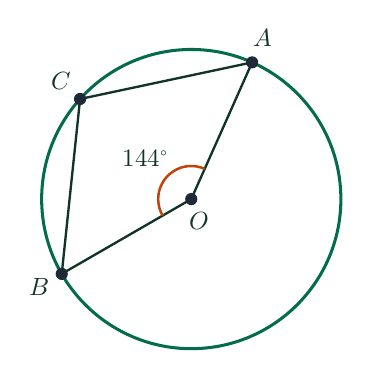
\begin{tikzpicture}
\draw[color={rgb,255:red,4;green,107;blue,77}, line width=1.1pt] (0,0) circle (1.900);
\draw[ink, line width=0.85pt] (-1.412,1.271) -- (0.773,1.736);
\draw[ink, line width=0.85pt] (-1.412,1.271) -- (-1.645,-0.950);
\draw[ink, line width=0.85pt] (0.000,0.000) -- (0.773,1.736);
\draw[ink, line width=0.85pt] (0.000,0.000) -- (-1.645,-0.950);
\draw[color={rgb,255:red,194;green,65;blue,12}, line width=0.9pt] (0.171,0.384) -- (0.121,0.402) -- (0.070,0.414) -- (0.018,0.420) -- (-0.035,0.419) -- (-0.087,0.411) -- (-0.138,0.397) -- (-0.187,0.376) -- (-0.232,0.350) -- (-0.274,0.318) -- (-0.312,0.281) -- (-0.345,0.240) -- (-0.372,0.195) -- (-0.394,0.146) -- (-0.409,0.096) -- (-0.418,0.044) -- (-0.420,-0.009) -- (-0.415,-0.061) -- (-0.405,-0.113) -- (-0.387,-0.163) -- (-0.364,-0.210);
\node[font=\small, text=ink, inner sep=0.5pt, fill=white] at (-0.580,0.522) {$144^\circ$};
\fill[color={rgb,255:red,31;green,41;blue,55}] (0.773,1.736) circle (2.2pt);
\fill[color={rgb,255:red,31;green,41;blue,55}] (-1.645,-0.950) circle (2.2pt);
\fill[color={rgb,255:red,31;green,41;blue,55}] (-1.412,1.271) circle (2.2pt);
\fill[color={rgb,255:red,31;green,41;blue,55}] (0.000,0.000) circle (2.2pt);
\node[font=\small, text=ink, inner sep=0.5pt] at (0.911,2.046) {$A$};
\node[font=\small, text=ink, inner sep=0.5pt] at (-1.940,-1.120) {$B$};
\node[font=\small, text=ink, inner sep=0.5pt] at (-1.665,1.499) {$C$};
\node[font=\small, text=ink, inner sep=0.5pt] at (0.103,-0.282) {$O$};
\end{tikzpicture}
\end{document}
